\documentclass[12pt,twoside]{report}% Use this line for the print version of the thesis
%\documentclass[12pt,oneside]{report}% If you comment out the line above, and uncomment this line, it will create a file without the extra pages that the Library wants for its electronic file versions.

\usepackage{byustyle}
\byustylesetup{%
    % Definitions of names needed in thesis/dissertation
    deptname          = School of Technology,
    committeechairman = Barry Lunt,
    committeemembera  = Derek Hansen,
    committeememberb  = Richard Helps,
    %graddate = April 2011,  		% Final approval month (NOT graduation month!
     %
    %Uncomment to shorten for proofreading purposes
    %noabstract = true,         % Don't show the abstract page
    %nouniversitypages = true,  % Don't show any of the "university pages"
    %noacknowledgements = true, % Don't show the Acknowledgements page
    %notableofcontents = true,  % Don't show the Table of Contents
    %nolistoffigures = true,    % Don't show the List of Figures
    %nolistoftables = true,     % Don't show the List of Tables
    %nonomenclature = true,     % Don't show the Nomenclature section - note that this section is optional
    %notocandlists = true,      % Don't show the Table of Contents, List of Figures, or the List of Tables
    %noheaderatall = true,      % Don't show any of the BYU Thesis header pages
    keywords = {David Kolb, LSI, computing, academic success, AMSS} % Enter your keywords
%inside the curly braces, as you'd like them to appear on the bottom of the abstract page.
}

%%%%%%%%%%%%%%%%%%%%%%%%%%%%%%%%%%%%%%%%%%%%%%%%%%%%%%%%
%  Include other \usepackage{} statements here.
%    Add one package at a time.
%    Warning:  Some packages are not compatible with byuthesis.sty
%%%%%%%%%%%%%%%%%%%%%%%%%%%%%%%%%%%%%%%%%%%%%%%%%%%%%%%%%
% You should turn on any of these that you think you'll need!

%\usepackage[normalmargins]{savetrees} 	% prints smaller to save trees (draft only)
\usepackage{amsmath}										%	allows for mathematical symbols
\usepackage{amssymb}										%	defines symbol names for all the math symbols
\usepackage{graphicx}        						% for .pdf graphics inclusion
\usepackage{caption}
\usepackage[calcwidth = \columnwidth]{caption}
\usepackage{booktabs,threeparttable}
\usepackage{subcaption}
\usepackage{setspace}										%	change the spacing inside a document
\usepackage{epstopdf}										%	converts a .eps to a .pdf
\usepackage{cite}												%	allows for citations
\usepackage{mathptmx}
\usepackage{textcomp}
\usepackage{float}											%	improves the interface for defining floating objects
\usepackage{rotating}
%\usepackage[figuresright]{rotfloat}
%\usepackage{multirow}
%These next two lines are for the citing with the IEEE style (leave commented for ASME)
%\renewcommand\citepunct{], [}
%\renewcommand\citedash{]--[}

% %%%%%%%%%%%%%%%%%%%%%%%%%%%%%%%%%%%%%%%%%%%%%%%%%%%%%%%
% For doing bookmarks in the PDF file
% %%%%%%%%%%%%%%%%%%%%%%%%%%%%%%%%%%%%%%%%%%%%%%%%%%%%%%%
% For more info, see:
% http://www.geocities.com/kijoo2000/latex2pdf.pdf
% http://www.tug.org/applications/hyperref/manual.html
\usepackage[pdftex,backref=false,pagebackref=false,plainpages=false]{hyperref}
\hypersetup{
  breaklinks   = false, % Allow link text to break across lines (default=false).
  linktocpage  = false, % make page number, not text, be link on TOC, LOF and LOT
  colorlinks   = false, % Color the text of links (true) or put color frames over
  %
  linkbordercolor  = {1 1 1}, % The color of the box around normal links (white so they won't show up)
  citebordercolor  = {1 1 1}, % The color of the box around citations (white so they won't show up)
                        % the links (false).
  pdfstartview = {FitV}, % Set the startup page view. Possible options are:
                         % FitH: Fit whole width of page
                         % FitV: Fit whole height of page
                         % FitB: Fit whole �Bounding Box� page
                         % FitBH: Fit whole width of �Bounding Box� of page
                         % FitBV: Fit whole height of �Bounding Box� of page
  bookmarksnumbered  = true, % Put section numbers in bookmarks (default=false)
  bookmarksopen      = true, % Open up the bookmark trees (default=false).
  bookmarksopenlevel = 0, % Level to which bookmarks are open (default=\maxdimen).
  bookmarkstype      = toc, % Specify which toc file to mimic (default=toc).
  pdfpagemode        = {UseOutlines}, %  Specify how document starts when opened ({None}).
                                      % Possible options are:,
                                      % None: Neither bookmarks nor thumbnails are visible.
                                      % UseOutlines: Bookmarks are visible.
                                      % UseThumbs: Thumbnails are visible.
                                      % FullScreen: Full-screen mode
  pdftitle    = {Thesis},
  pdftitle    = {A Cognitive Approach to Predicting Academic Success in Computing},
  pdfauthor   = {Colby Goettel},
  pdfcreator  = {Colby Goettel},
  pdfsubject  = {Colby Goettel's Master's Thesis},
  pdfkeywords = {Master's Thesis, BYU, computing, academic success, lsi},
  pdfborder		=	{0 0 0},
}

\usepackage[round]{natbib}

%%%%%%%%%%%%%%%%%%%%%%%%%%%%%%%%%%%%%%%%%%%%%%%%%%%%%%%%
%  Define macros here - You may use these, or delete them, as you see fit.
%%%%%%%%%%%%%%%%%%%%%%%%%%%%%%%%%%%%%%%%%%%%%%%%%%%%%%%%%
\newcommand{\norm}[1]{\left\|#1\right\|}
\newcommand{\abs}[1]{\left|#1\right|}
\newcommand{\defeq}{\stackrel{\triangle}{=}}
\newcommand{\re}{\mathbb{R}} 																			% real numbers
\newcommand{\OMIT}[1]{{}} 																				% omit sections of text
\newcommand{\pd}[2]{\ensuremath{\frac{\partial #1}{\partial #2}}} % partial derivative
\newcommand{\superscript}[1]{\ensuremath{^\textrm{#1}}}
\newcommand{\subscript}[1]{\ensuremath{_\textrm{#1}}}

\DeclareCaptionJustification{InvertedPyramid}{\hsize=\linewidth
                \parindent=0pt
                \leftskip=0pt plus.5fil
                \rightskip=0pt plus-0.5fil
                \parfillskip=0pt plus1fil
                \emergencystretch=1in
                \parshape10
                0.00in \linewidth
                0.025\linewidth 0.95\linewidth
                0.05\linewidth 0.9\linewidth
                0.075\linewidth 0.85\linewidth
                0.1\linewidth 0.8\linewidth
                0.125\linewidth 0.75\linewidth
	     0.15\linewidth 0.70\linewidth
	     0.175\linewidth 0.65\linewidth
	     0.2\linewidth 0.60\linewidth
	     0.225\linewidth 0.55\linewidth
                \strut
	}
\renewcommand{\TPTminimum}{3in}
\captionsetup[table]{justification=InvertedPyramid}

\newsavebox{\tempbox}
\newlength{\tempwidth}

% %%%%%%%%%%%%%%%%%%%%%%%%%%%%%%%%%%%%%%%%%%%%%%%%%%%%%%
% To only print a few chapters without changing the reference numbers,
%	uncomment the chapters you want
% %%%%%%%%%%%%%%%%%%%%%%%%%%%%%%%%%%%%%%%%%%%%%%%%%%%%%%
%\includeonly{chapter1}
%\includeonly{chapter2}
%\includeonly{chapter3}
%\includeonly{chapter4}
%\includeonly{chapter5}
%\includeonly{chapter6}
%\includeonly{chapter7}
%\includeonly{appendixa}
%\includeonly{appendixb}
%\includeonly{appendixc}
%\includeonly{appendixd}

%%%%%%%%%%%%%%%%%%%%%%%%%%%%%%%%%%%%%%%%%%%%%%%%%%%%%%%%
% Start Document
%%%%%%%%%%%%%%%%%%%%%%%%%%%%%%%%%%%%%%%%%%%%%%%%%%%%%%%%
\begin{document}

% Define Title & Author
% For a title of more than one line, use the \\ to break up the lines so they appear in an inverse pyramid shape.
%Also, make sure you use title case (upper case for most of the first letters of words)
\title{A Cognitive Approach to Predicting\\Academic Success in Computing} %Ira A. Fulton College\\ of Engineering and Technology}
\author{Colby Goettel}

% For displaying the BYU Thesis header
% 	This command assumes that there are documents called abstract.tex and
% 	acknowledgements.tex that will be included in the header
\showBYUHeader

% Include chapters of the thesis here: (Note that you should open the files chapter1.tex and chapter2.tex to
% see some of the important notes about how to do your thesis!)
\chapter{Introduction}\label{chp:chapter1}
Incoming freshmen struggle deciding which field they should enter. In computing, there are many fields to choose from and this can cause confusion for new students, especially because the fields are so closely related. For example, many students don't know the difference between computer science (CS), information systems (IS), and information technology (IT). It would be so nice to have a simple way to determine which field would best suit the student. But how do these fields differ? And how do these differences help us determine the right fit for incoming computing students?

One potential way to look at the differences among the various computing fields is to look at the characteristics of the students in each of these fields~--- especially how they prefer to learn. CS, IS, and IT all focus on different areas of computing and each requires a different skill set. Is it possible to predict in which computing discipline an incoming freshman would succeed based on their learning style preferences? Previous research has shown a correlation between learning preference and academic success for engineering students (Lunt, 1996), but does this correlation also exist for computing students?

In the early 1970s, Dr.\ David Kolb developed a cognitive model to represent learning preferences. His model works on a two-axis system: concrete experience (CE) versus abstract conceptualization (AC), and reflective observation (RO) versus active experimentation (AE). This two-axis spectrum is meant to describe a student's learning preferences.

The \textit{x}-axis, AE$-$RO, differentiates between students who prefer to learn by doing, being active, seeing results, and those who prefer to learn by watching, listening, taking their time, and relying on observations. The \textit{y}-axis, AC$-$CE, differentiates between students who prefer to learn by thinking things out, reasoning, being rational, and those who are more intuitive and prefer to trust their feelings.

It doesn't appear that any research has been done in this area, \textit{viz}.: examining if a student's cognitive learning preference is a factor in which computing discipline they should study. Some of the research is close, but most deal with programming aptitude or success in a first year program. Interestingly, hardly any research has taken a cognitive approach. Finally, no research was found that focused on the differences between CS, IS, and IT.

\section{Purpose}
The purpose of this research is to discover if there is a correlation between a student's preference for AC$-$CE and AE$-$RO and their GPA, and overall satisfaction in CS, IS, and IT. This research matters because incoming freshman interested in computing struggle to decide between the various, computing majors. If there is a statistically significant correlation between Kolb's learning styles and success in CS, IS, and IT, then advisement centers could use the LSI to help incoming students choose among computing majors.

\section{Research questions}
\begin{itemize}
  \item How strong is the correlation between AC$-$CE and AE$-$RO, and major GPA among CS, IS, and IT students?
  \item How strong is the correlation between AC$-$CE and AE$-$RO, and student satisfaction among CS, IS, and IT students?
  \item Is there a correlation between major GPA and student satisfaction?
  \item What is the best multiple regression model to fit these correlations?
\end{itemize}

\section{The computing disciplines}
The Association for Computing Machinery (ACM) has defined five disciplines in computing~(Shackelford, 2006): computer engineering, computer science, information systems, information technology, and software engineering. Although there is overlap between disciplines, each discipline fills its own niche. Computer engineering is focused on designing and building computer hardware and its associated software. Computer science creates low-level software, and is also concerned with the theoretical principles of computing. Software engineering is primarily focused on creating highly reliable software systems. Information technology solves general computer problems and fulfills the organizational need to integrate systems. Information systems also fulfills an organizational need, but mostly from the management side.

\section{What is cognition?}
David Kolb created the Experiential Learning Theory (ELT)~(Kolb, 2005a) and used this theory as the basis for his Learning Style Inventory (LSI). This theory has its roots in famous cognitivists and learning philosophers like Dewey, Piaget, Jung, Freire, and Carl Rogers.

Kolb said that ``[l]earning is best conceived as a process, not in terms of outcomes''~(Kolb, 2005a). In this view, learning is more about the journey than the outcome. This is important because the ELT focuses on how ``[l]earning is the process of creating knowledge''~(Kolb, 2005a). This view is based on the Constructivist Theory of learning which says that a learner must construct new knowledge, or as Kolb said, ``[S]ocial knowledge is created and recreated in the personal knowledge of the learner''~(Kolb, 2005b). It's contrasted with the Transmission Model whereby ``pre-existing fixed ideas are transmitted to the learner''~(Kolb, 2005a).

This might seem like a purely semantic difference, but there's an important distinction between constructivism and transmission, much like there's an important distinction between learning as a process and learning as the end result. This is important because the ELT and this research focus on learning as a process: it matters \emph{how} students learn, not simply \emph{what} they learn.

\section{What is satisfaction?}
Satisfaction is how pleased a student is with their major decision. In order to be quantified, satisfaction was rated by the Academic Major Satisfaction Scale which was developed and validated in 2007 by Margaret Nuata. It contained questions that asked the student to rate how happy they were with their major, if they considered changing majors, and how they felt about their major:
\begin{enumerate}
  \item ``I often wish I hadn't gotten into this major.
  \item I wish I was happier with my choice of an academic major.
  \item I am strongly considering changing to another major.
  \item Overall, I am happy with the major I've chosen.
  \item I feel good about the major I've selected.
  \item I would like to talk to someone about changing my major''~(Nuata, 2007).
\end{enumerate}

\section{Delimitations}
This research was limited to seniors because they have been exposed to myriad professors and courses, giving them a well-rounded view of the institution. Furthermore, this research was limited to CS, IS, and IT students at BYU because there are too many confounding variables to properly deal with other schools and their admissions processes in a study of this size.

This research did not look at the socioeconomic backgrounds of the students involved. It did not consider any social pressure students may receive to join a particular field.

\chapter{Literature review}\label{chp:chapter2}
The literature review focused on studies already done on this topic, how previous studies in computing had incorporated cognitive theory, and what surveys should be used to assess a student's cognitive learning preference and their satisfaction with their major.

The literature review was performed through Google Scholar and Brigham Young University's Harold B.\ Lee Library website. The criterion for a study to be considered relevant was that it had to match at least one of the following criteria:
\begin{enumerate}
  \item The study had to be about predicting academic success of students. For initial research, the tools and measures were not important. Once the author had an idea of which tools to use, further research was done on the reliability and efficacy of the given tools, as well as research into any criticism of those tools.
  \item For studies involving cognitive learning preferences, the studies were limited to science, technology, engineering, or mathematics (STEM) majors. For studies on criticism of the research tools, the search was expanded to include other disciplines because of the lack of relevant studies among the computing disciplines.
  \item The study had to be on students, not organizations. Additionally, the study could not be on a specific demographic subgroup of students (e.g., only 21 year-old Asian students whose parents have PhDs). Some studies were performed in niche environments and those qualities are noted in the following reviews.
  \item There was no requirement for the study to examine previous experience, high school performance, or tools like the SAT or ACT.
\end{enumerate}

The initial literature review was to find studies related to cognitive learning preference and how it affected STEM students. Upon finding that there was bountiful research in the area, the literature review was focused on finding studies related to cognitive preference among STEM students. Then, the literature review was expanded to include studies on academic success. Finally, the literature review focused on tool validation.

\section{Learning theories}
\subsection{Top-down and bottom-up}
In 2003, Ron Sun published a paper entitled Top-down versus bottom-up learning in cognitive skill acquisition(Sun, 2004). This paper looked at two different cognitive learning styles. These styles, respectively, were about whether acquiring knowledge was from a general idea to a specific idea, or vice versa. As important as this idea is, Sun's paper had no independent research to back it up.

\subsection{Acquisition and participation metaphors}
Sfard mentioned two metaphors for learning~(Sfard, 1998): acquisition metaphor (AM) and participation metaphor (PM). AM says that people learn by learning (as opposed to doing). Facts, ideas, and concepts build on each other. These pieces of information~--- referred to as objects~--- are colloquially known as knowledge. Knowledge is then internalized and stored in memory. Historically, AM has been the metaphor used for thousands of years to describe knowledge and learning. Generally, when people think about learning, they are thinking about the AM.

PM is a learning style dictated by actions: people learn by doing. PM advocates teach that knowledge is not something that people have, it's societal and communal: learning is done by being part of a community. This type of learning is all-encompassing, meaning that learning isn't something that someone has, it's one part of the whole.

\subsection{Atkinson-Shiffrin model of memory}
\begin{figure}
  \centering
  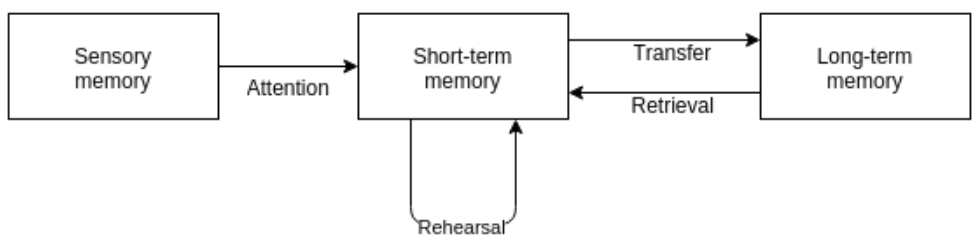
\includegraphics[width=\textwidth]{figures/chapter2/atkinson-model-of-memory.png}
  \caption{The Atkinson-Shiffrin Model of Memory}
  \label{fig:atkinson-model-of-memory}
\end{figure}

The Atkinson-Shiffrin model of memory is shown in Figure~\ref{fig:atkinson-model-of-memory}. The premise is that as individuals pay attention to sensory stimulation, short-term memories are created. As short-term memory is rehearsed and transferred, it turns into long-term memory. As long-term memory is retrieved, it comes into short-term memory so that it can be used.

The major components of this model are some form of input, storage, retrieval, and (eventually) forgetting. When presented with information, an individual must input and store the information. This creates short-term memory. If this memory is rehearsed (retrieved) often, it has a chance to become long-term memory. Neurologically speaking, when memories are rehearsed, the myelin sheaths of neurons form along certain pathways making memory. However, like muscle, if these memories are not used, they are lost.

This model works as a basic model of human learning because learning is the internalization of knowledge in long-term memory. If an individual has successfully internalized and retrieved knowledge, they have learned. In education, this is the predominant reason why exams exist: exams test students to see if they have learned the concepts taught in a class.

The Atkinson-Shiffrin model of memory shows the basic process by which people store information, but lacks the depth necessary to properly portray pedagogy. Learning is more than memorization: it's also internalization and application.

\subsection{Vygotsky's learning models}
According to Vygotsky~(Vygotsky, 1978), learning is not something people have, it's something they do. Learning is participatory. It is experiencing something that happened in the world. This is incredibly close to how David Kolb defined learning: ``[T]he process whereby knowledge is created through the transformation of experience''~(Kolb, 2013).

In contrast to learning, development is the actual progress being made by the learner. Development is the fruits of learning. In Vygotsky's mind, there are two types of development: actual development and proximal development. Actual development is what a learner can do. Proximal development, however, is the distance between what a learner can do on their own versus what they can do with someone more knowledgeable than themselves. This more knowledgeable person is not necessarily a master of their domain, but a peer or a teacher — they just have to be someone more knowledgeable in the learner's domain.

Vygotsky theorized that learning is experiences had in the world: learning happens all the time. In fact, everyone in the world that directly or indirectly influences the learner contributes to learning. This idea of communal learning, influenced by Marxism, is the idea that learners interact with others who already know how to live in the society; and learners learn how to live in their society through these interactions. Communal learning makes up a huge part of Vygotsky's idea of cultural apprenticeship, apprenticeship having more to do with interacting than coaching.

Because Vygotsky came from a communist nation, his thinking is heavily influenced by Marxist ideas. A prevalent, Marxist idea at his time was called Sovietization: if you can make someone live like a communist, they will think like a communist. This worked right into Vygotsky's collectivist thinking and influenced his ideas on social reproduction and enculturation: we become like the community when we learn to think and act like them. This cultural learning is not restricted to schooling because a lot of learning happens outside of school and especially before formal schooling begins. Children begin learning long before school: learning about their culture, their surroundings, their family.

Vygotsky thought of learning as a verb, not a noun: learning is not necessarily something that is had, it's something that is done. This works perfectly into the participation metaphor. He theorized that development is what a child is capable of doing: development is the fruit of learning. Vygotsky believed that what a child can do with others is more indicative of their development than what they can do alone.

Vygotsky was so radically different than his predecessors that he started an entire movement. The idea that learning is what influences development was in stark contrast to previous theorists who either believed that development came first or that learning and development were intertwined. Vygotsky changed the way people think about learning and was hugely influential in informing the learning theories used in this research.

\subsection{Experiential Learning Theory}
The Experiential Learning Theory (ELT), a cognitive approach to learning, was started by David A. Kolb in the 1970s and has continued to be updated with modern research since~(Kolb, 2005a). This theory and its related survey, the Kolb Learning Style Inventory (LSI), have been used and validated repeatedly since their creation. In fact, the survey is currently in its fourth major release.

Kolb says that ``[l]earning is best conceived as a process, not in terms of outcomes''~(Kolb, 2005a). In this view, learning is more about the journey than the outcome. This is important because the ELT focuses on how ``[l]earning is the process of creating knowledge''~(Kolb, 2005a). This view is based on the Constructivist Theory of learning which says that a learner must construct new knowledge, that is to say, ``[S]ocial knowledge is created and recreated in the personal knowledge of the learner''~(Kolb, 2005b). It's contrasted with the Transmission Model whereby ``pre-existing fixed ideas are transmitted to the learner''~(Kolb, 2005a).

This might seem like a purely semantic difference, but there's an important distinction between constructivism and transmission, much like there's an important distinction between learning as a process and learning as the end result. This is important because the ELT and this research focus on learning as a process: it matters how students learn, not simply what they learn. For these reasons, the ELT was chosen as the basis for assessing cognitive preference.

\section{Related studies}
\subsection{Lunt's \textit{Predicting Academic Success in Electronics}}
Lunt's dissertation, \textit{Predicting Academic Success in Electronics}~(Lunt, 1996), was foundational for this thesis. It performed the same research being performed here, but with an older version of the Kolb Learning Style Inventory (LSI), a focus on the electronics fields, and no focus on major satisfaction.

The purpose of Lunt's research was to determine if there was a correlation between learning style preference and academic success in electronics technology, electronics engineering technology, and electrical engineering. If there was a statistically significant correlation, then the LSI could be used as an accurate discriminator to help students choose in which electronics program they should enroll.

The students were randomly sampled and there was a participation rate of 45\%. Because the students were randomly sampled and the participation rate was $>$10\%, inferences to the population could be drawn.

The research questions were:
\begin{enumerate}
  \item ``What are the best predictor variables for predicting academic success in electronics?
  \item Is abstract learning preference an effective discriminator between students in the three main types of electronics programs?
  \item What is the best multiple-regression model that can be derived for predicting success in each of the three types of electronics programs?''~(Lunt, 1996)
\end{enumerate}

This rationale was persuasive because it focused on the differences between various majors in the same field and it was aimed at helping students determine which major to choose. Additionally, the Kolb LSI is a tested and validated tool for determining cognitive preference. Finally, the Experiential Learning Theory (ELT) on which the test is based fits right in line with the ideas behind this research.

The multiple regression model presented found correlations which helped justify the need to expand this line of research to computing students.

The paper's claims were justified in light of the methods used and it drew many interesting implications. This paper found that AC-CE~--- a Kolb axis measured by the LSI~--- is a good discriminator and can be used to help potential electronics students choose a major.

\subsection{Other studies}
There were several non-cognitive studies~(Thomas, 2007; Elnagar, 2013; Ridgell, 2004; Ting, 2001) that were foundational in understanding the scope of research done in this field. Other studies focused on previous academic success~(Barlow-Jones, 2011; Golding, 2005; Ting, 2001; Campbell, 1984), programming or mathematics aptitude~(Nowaczyk, 1984; Evans, 1989), or other unrelated and non-cognitive models~(Barlow-Jones, 2011; Elnagar, 2013).

The most common non-cognitive tool used was the Non-Cognitive Questionnaire (NCQ); however Thomas found that ``none of the scales of the NCQ are adequate predictors of GPA or persistence in college''~(Thomas, 2007). Other non-cognitive tools included personality tests (e.g., Myers-Briggs Personality Type Indicator, 16 Personality Test), general knowledge tests (e.g., SAT, ACT), and work drive. In 2004, Ridgell studied these variables with great success ($p<0.01$) finding that the personality traits exam was found to statistically correlate with course grades and GPA. However, none of the tools Ridgell used were cognitively-based.

In the same vein, \textit{Predicting Academic Performance in the School of Computing \& Information Technology (SCIT)}~(Golding, 2005) looked at students' performance in first-year courses. This was useful because it looked at all courses a first-year student takes, not just programming courses as most studies did. The study also looked at demographic information and a student's qualification for entry to the school and aptitude test scores, neither of which are administered in the US. It then used these indicators, as well as a student's overall performance in the program, to predict their future performance. However, the study did not look at college entrance exam scores or high school GPA. This research found that none of the entrance exams used~--- including the SAT~--- were good predictors for academic success. It also found that high school success in math, science, and previous IS and IT classes were not good indicators for academic success. Mostly, this paper found that the then-current indicators for admission were incorrect and not statistically significant. The only positively-correlated finding was that first-year programming and networking classes were good indicators for later success~(Golding, 2005).

Historically, studies tried to determine academic success by a student's programming or math aptitude using surveys like the Fennema-Sherman Mathematics Attitude Scale~(Nowaczyk, 1984), the IBM Programmer Aptitude Test~(Hostetler, 1983), or even COBOL~(Nowaczyk, 1984) or FORTRAN~(Campbell, 1984) proficiency. However, these surveys were found to not be the most effective tools to determine future academic success with ``R-squares of less than 24 percent''~(Evans, 1989).

\section{Why cognition?}
The various studies already mentioned each take a non-cognitive approach to predicting academic success. Since previous studies have failed to look at cognition, it leaves a clear opportunity that this research can fill. Cognition might not be the right theory, but that needs to be addressed. Additionally, cognitive theory seems to be the best candidate because it focuses on how students think and interpret information which is key in understanding technical concepts.

\section{Cognitive learning preference}
In 2005, the Hay Group published \textit{Learning Styles and Learning Spaces: Enhancing Experiential Learning in Higher Education} which gave interpretations about the various learning styles in the LSI. This paper was useful because it is the foundation of some hypotheses, namely that CS and IS will be in different quadrants of the LSI. IT was not listed, although it falls roughly, but not squarely, into engineering. Since CS and management are in different quadrants, and IS is the management side of technology, it would follow that IS should probably be in a different quadrant. However, no information has been found supporting this claim so it's an important claim to test.

\section{Criticism of the LSI}
In 1990, DeCoux surveyed cognitive research on nursing students that used the LSI. This was done in an effort to determine if the LSI was a trusted assessment tool. DeCoux's research showed ``a lack of significant relationships between learning style and other variables,'' adding further that ``studies undertaken specifically to investigate the measurement properties of the LSI reported major criticisms which seem to have been ignored.'' Throughout the survey, DeCoux found that the LSI was ``the most frequently used method of measuring learning styles'' even though there were ``numerous charges of serious instrument weakness,'' concluding that ``[c]ontinued use of the Kolb LSI... as an experiential technique is not recommended''~(DeCoux, 2016).

More recent research has shown that ``[d]ifferent personality traits... and academic motivation... were found to be independently associated with student learning strategies''~(Donche, 2013). This study, covering more than 1,100 undergraduate students, found that teaching strategy was hugely impactful because of ``the importance of students' personality and academic motivation'' which were found to ``partly explain'' how students learn.

Despite these criticisms, the LSI has been widely used in previous research in this area and is still generally considered to be a valid learning style assessment tool. Most of the studies looked at as part of this literature review did not have negative things to say about the LSI, although they were not looking into the tool's validity. For these reasons, we have decided to adopt the LSI as the learning style assessment tool.

\section{Criticism of cognition and learning styles}
Wang and others looked into the correlation between Biggs' constructive alignment and how it affected students' learning approaches. This research went off the basis that ``university students' learning approaches... are highly correlated with students' achievement of learning outcomes''~(Wang, 2013). However, it then noted that ``[s]uch a statement... was underpinned neither by qualitative nor quantitative empirical data.'' Their research showed that a more constructively-aligned teaching environment ``would lead students to adjust their learning approaches'' so they could learn more deeply ``despite their pre-existing individual differences in the preferred learning approaches.'' Their research is important because it showed that learning preference, while not insignificant, could be forgone in order to learn deeply.

One of the main motivations fueling this research was the author's experience in IT and CS classes and how they so greatly differed. Because of the attitudes of the students in each major toward their courses and how the courses were taught, the author hypothesized that the cause of this schism was the learning styles of the students, so the author wished to pursue research in that realm.

\section{Defining satisfaction}
To assess student major satisfaction, Nuata's Academic Major Satisfaction Scale (AMSS) was used. Nuata created and validated this 6-item assessment in 2007 for her dissertation because there didn't seem to be an existing survey, noting that ``[s]urprisingly, studies investigating major satisfaction are fairly infrequent in the career-development literature''~(Nuata, 2007).

Over the course of her research, Nuata went through multiple iterations before landing on the six questions in the AMSS. After her first methodology which was comprised of 20 Likert-type questions, Nuata reformulated the AMSS into six Likert-type questions and found that ``[a]mong this new sample, Cronbach's alpha for the 6 AMSS items was .90. As in Study 1, this suggested that the items comprising the AMSS are fairly internally consistent''~(Nuata, 2007). Then in 2014, the AMSS was adapted for Korean students and re-validated~(Sovet, 2014). This helped show that the AMSS is a realistic and reliable tool for determining major satisfaction.

\section{Conclusion}
The literature was severely lacking in cognitive studies in computing. Every study found took a non-cognitive approach, looked at programming aptitude, or tried to use previous academic success and aptitude tests to predict future academic success. Furthermore, the literature almost exclusively focused on CS with IT and IS being either completely overlooked or an afterthought. This study helps fill the gap in research by providing a look into the cognitive learning preferences of computing students. Since there is no clear way to successfully predict academic success in computing, this research will help fill that gap by exploring a new avenue to predict academic success in computing.


% Bibliography
\cleardoublepage
\bibliographystyle{chicago}%Change this to use a different bibliography style, such as ieeetr.
\nocite{*}
\bibliography{master}% Change this to use a different bibliography database file.

% Appendices
\appendix
\chapter{R Code for Data Analysis}
\label{apdx:appendixa}
\lstinputlisting[language=R]{data_analysis.R}

\chapter{Formatting Guidelines for Thesis}
\label{apdx:appendixb}

This appendix outlines the required formatting for theses and dissertations. While the \LaTeX\ template takes care of most of these automatically, it is the student's responsibility to ensure that all formatting requirements are incorporated in the document.

\section{Font} Times New Roman 12 pt. throughout text and 10 or 11 point for tables and figures.

\section{Margins}
\begin{itemize}
\item Preliminary Pages (Title page, Abstract page(s), Acknowledgment page, Table of Contents, List of Figures, List of Tables):
1 inch on all sides
\item Body Pages, beginning with Introduction:
1 inch on all sides
\item Chapter title pages, Appendix title page, Reference title page:
2 inches at top,
1 inch at bottom and sides
\end{itemize}

\section{Printing}
\begin{itemize}
\item Single-sided: Title page, Abstract page(s), Acknowledgment page
\item Two-sided:  Table of Contents, List of Figures, List of Tables, Body, Appendix, References
\end{itemize}
Note:  Table of Contents, List of Figures, List of Tables, Chapter title pages, References and Appendix pages must begin on the front side of a page.

\section{Page Numbering}
\begin{itemize}
\item	Page numbers are centered at the bottom of the page.
\item	Counting begins with the Title page; however, back pages are not counted until the Table of Contents.
\item	Page numbers do not appear on the page until the Table of Contents (v).
\item	Use Roman Numerals (v, vi, vii, ...) for the Table of Contents page and the pages thereafter until Chapter 1.  
\item	Use Arabic numbers (1, 2, 3 ...) beginning with Chapter 1. 
\item	Be sure numbers appear on all blank back pages once numbering begins.
\end{itemize}

\section{Spacing}
\begin{itemize}
\item	Double-space text of body.
\item	Single-space abstract, captions, quotes, long chapter titles, headings, and subheadings.
\item	Table of Contents, List of Figures, List of Tables, and References can be single-spaced or double spaced.
\item	Double-space three times after chapter titles (48 pts).
\item	Double-space twice before subheadings (24 pts). 
\item	Double-space once after subheadings (0 pts). 
\item	Double-space once between two subheadings (0 pts). 
\item	Double-space twice before and after figures (24 pts).
\item	Double-space twice before and after tables (24 pts).
\item	Double-space once before and after equations (0 pts).
\item	Do not leave a single line of text, a single-line equation, or a subheading alone on the top (widow) or bottom (orphan) of a page.
\item	Do not leave more than about 5 lines of white space remaining on a page unless it�s the end of a chapter.
\end{itemize}

\section{Figures}
\begin{itemize}
\item	Figures are normally diagrams, graphs, maps, or charts.
\item	Center figures on the page.
\item	Center captions below the figure. If two lines are needed, the caption should be left justified at margin.
\item	A figure should be placed after the paragraph of reference.  If it will not fit on the same page, continue the text and place the figure on the next page.
\end{itemize}

\section{Tables}
\begin{itemize}
\item	Tables contain numerical or statistical information.
\item	Center tables on the page.
\item	Center captions above the table.  If more than one line is needed, center the lines in an inverted pyramid:                                                          
\begin{singlespace}
\begin{center}Table 6.3 Comparison of roll rotation plots when node was displaced,\\
 and an X-direction off-axis force was applied.\end{center}
\end{singlespace}
\item	If placed in the landscape position, the top of the table should be on the left side of the page, with the caption above the table.  The page number is placed in the standard location.
\end{itemize}

\end{document}
